% !TeX program = xelatex
%%%%%%%%%%%%%%%%%%%%%%%%%%%%%%%%%%%%%%%%%%%%%%%%%
% ACOSUS Paper: DSI 2026 revision
%%%%%%%%%%%%%%%%%%%%%%%%%%%%%%%%%%%%%%%%%%%%%%%%%

\documentclass[letterpaper,11pt]{article}
\usepackage[margin=1in]{geometry}
\usepackage{xurl}
\usepackage{graphicx}
\usepackage{alltt}
\usepackage{amsmath}
\usepackage{booktabs}
\setlength{\tabcolsep}{4pt}
\usepackage[hidelinks]{hyperref}
\hypersetup{pdftitle={ACOSUS: Design and feasibility evaluation of a structured advising platform for transfer students},pdfauthor={Deep Mandloi, Lizi Zhu, Xiwei Wang}}
\usepackage{float}
\usepackage{fontspec}
\IfFontExistsTF{Arial}{\setmainfont{Arial}}{\setmainfont{TeX Gyre Heros}}
\usepackage{fancyhdr}
\setlength{\headheight}{14pt}
\pagestyle{fancy}
\fancyhf{}
\fancyhead[C]{\makebox[\textwidth]{Mandloi et al.\hfill ACOSUS design and feasibility evaluation}}
\renewcommand{\headrulewidth}{0.4pt}
\renewcommand{\footrulewidth}{0pt}

% Float placement: let large figures/tables share a page with text instead of
% being banished to their own near-empty float pages.
\renewcommand{\topfraction}{0.9}
\renewcommand{\bottomfraction}{0.9}
\renewcommand{\textfraction}{0.08}
\renewcommand{\floatpagefraction}{0.75}
\setcounter{topnumber}{3}
\setcounter{bottomnumber}{2}
\setcounter{totalnumber}{4}

% TikZ packages for diagrams
\usepackage{tikz}
\usetikzlibrary{shapes.geometric, arrows.meta, positioning, fit, backgrounds, calc}

% Define colors for diagrams
\definecolor{targetsurvey}{HTML}{FFF3E0}
\definecolor{factorsurvey}{HTML}{E3F2FD}
\definecolor{processing}{HTML}{F3E5F5}
\definecolor{outputgreen}{HTML}{E8F5E9}
\definecolor{stage1green}{HTML}{D4EDDA}
\definecolor{stage1border}{HTML}{28A745}
\definecolor{stage2yellow}{HTML}{FFF3CD}
\definecolor{stage2border}{HTML}{FFC107}
\definecolor{stage3blue}{HTML}{CCE5FF}
\definecolor{stage3border}{HTML}{007BFF}
\definecolor{framegray}{HTML}{F8F9FA}
\definecolor{frameborder}{HTML}{6C757D}
\definecolor{modelpink}{HTML}{FCE4EC}
% Colors for fig2 (Three-Stage Pipeline)
\definecolor{stage1}{RGB}{76,175,80}
\definecolor{stage2}{RGB}{255,152,0}
\definecolor{stage3}{RGB}{100,149,237}
\definecolor{inputred}{RGB}{183,28,28}
\definecolor{outputviolet}{RGB}{103,58,183}
\definecolor{pipelineborder}{RGB}{120,60,60}
% Colors for fig3 (Survey Processing)
\definecolor{surveyblue}{RGB}{66,133,244}
\definecolor{surveyboxfill}{RGB}{215,232,252}
\definecolor{processorange}{RGB}{234,67,53}
\definecolor{processboxfill}{RGB}{253,232,226}
\definecolor{processboxborder}{RGB}{230,150,100}
\definecolor{modelgreen}{RGB}{15,100,80}
\definecolor{modelboxfill}{RGB}{200,230,225}
\definecolor{modelboxborder}{RGB}{100,180,170}
% Colors for fig4 (System Architecture)
\definecolor{dblue}{RGB}{60,100,180}

% TikZ styles
\tikzset{
    surveybox/.style={rectangle, rounded corners=3pt, minimum width=2.2cm, minimum height=0.8cm, text centered, draw=black!60, font=\scriptsize, text width=2cm, align=center},
    groupbox/.style={rectangle, rounded corners=5pt, draw=black!40, thick},
    arrow/.style={-{Stealth[length=2mm]}, thick, black!70},
    dashedarrow/.style={-{Stealth[length=2mm]}, thick, black!50, dashed},
    stagebox/.style={rectangle, rounded corners=5pt, minimum width=3cm, minimum height=1.8cm, draw, thick, text width=2.8cm, align=center, font=\scriptsize},
    layerbox/.style={rectangle, rounded corners=3pt, minimum width=2cm, minimum height=0.6cm, text centered, draw=black!60, font=\tiny, text width=1.8cm, align=center},
}
\urlstyle{same}
\usepackage{csquotes}
\usepackage[style=apa, backend=biber, sortcites=true, sorting=nyt]{biblatex}
\DeclareLanguageMapping{english}{english-apa}
\addbibresource{submission/main-v4-ai-edit-references.bib}

\usepackage[english]{babel}

\usepackage{ragged2e}
\setlength{\RaggedRightParindent}{0pt}
\RaggedRight
\linespread{1.0}
\setlength{\parindent}{0pt}
\setlength{\parskip}{0pt}
\setlength{\emergencystretch}{3em}

\usepackage{titlesec}
% Level 1: ALL CAPS, bold, left-aligned, no displayed number
\titleformat{\section}{\normalfont\bfseries\MakeUppercase}{}{0pt}{}
% Level 2: bold, sentence case, no displayed number
\titleformat{\subsection}{\normalfont\bfseries}{}{0pt}{}
% Level 3: underlined, sentence case, not bold, no displayed number
\titleformat{\subsubsection}{\normalfont}{}{0pt}{\underline}
\titlespacing*{\section}{0pt}{1.5\baselineskip}{0.5\baselineskip}
\titlespacing*{\subsection}{0pt}{1\baselineskip}{0.5\baselineskip}
\titlespacing*{\subsubsection}{0pt}{0.5\baselineskip}{0.5\baselineskip}

\begin{document}
\thispagestyle{empty}
\noindent\makebox[\textwidth]{Mandloi et al.\hfill ACOSUS design and feasibility evaluation}\par
\vspace{2pt}
\hrule
\vspace{24pt}

\begin{center}
\textbf{DECISION SCIENCES INSTITUTE}\\[6pt]
% REV-TITLE-001 BEGIN: active design-and-feasibility title.
ACOSUS: Design and feasibility evaluation of a structured advising platform for transfer students
% Alternative A: ACOSUS: A structured advising and data collection platform for transfer students
% Alternative B: Designing ACOSUS: A transfer-student advising platform for structured data collection
% REV-TITLE-001 END
\\[12pt]
% Author metadata placeholders requested for the DSI final template.
Deep Mandloi\\
\textit{[Affiliation]}\\
\textit{[Complete address]}\\
\textit{[Email]}\\
\textit{[Telephone number]}\\[6pt]
Lizi Zhu\\
\textit{[Affiliation]}\\
\textit{[Complete address]}\\
\textit{[Email]}\\
\textit{[Telephone number]}\\[6pt]
Xiwei Wang\\
\textit{[Affiliation]}\\
\textit{[Complete address]}\\
\textit{[Email]}\\
\textit{[Telephone number]}
\end{center}

\bigskip
\begin{center}
\textbf{ABSTRACT}
\end{center}

% REV-ABSTRACT-001 BEGIN: 95-word design-and-feasibility abstract.
Transfer students face fragmented records and advising processes that often omit the academic and nonacademic context of transfer. We present ACOSUS, a structured advising platform linking outcome-oriented and factor surveys with advisor-visible student profiles. A feasibility pilot with ten transfer students from six public U.S. universities evaluated the survey workflow and student experience. Participants rated ease of use positively, while usefulness and behavioral intention varied. The pilot supports the feasibility of structured data collection and advisor-facing organization, not predictive validity. A post-pilot model diagnostic is reported and does not establish prediction of longitudinal student outcomes.
% REV-ABSTRACT-001 END

\bigskip

\noindent\textbf{KEYWORDS:}\quad transfer students, academic advising, information systems, technology acceptance, student persistence

%%%%%%%%%%%%%%%%%%%%%%%%%%%%%%%%%%%%%%%%%%%%%%%%%
% SECTION 1: INTRODUCTION
%%%%%%%%%%%%%%%%%%%%%%%%%%%%%%%%%%%%%%%%%%%%%%%%%
\section{Introduction}\label{sec:introduction}

Many students begin at community colleges and later transfer to four-year universities to complete their degrees. National studies estimate that more than one-third of undergraduates follow this route \parencite{monaghan2015}, and the proportion is even higher in computing and other STEM majors and among first-generation, low-income, and racially minoritized students \parencite{computingtransfer2024,wali2025transfer}. Although this pathway offers a more affordable route to a bachelor's degree \parencite{factoranalysis2023}, it also creates coordination problems between sending and receiving institutions \parencite{nguyen2025school}. Advisors must work with articulation agreements, uneven credit recognition, and limited access to students' pre-transfer coursework \parencite{nguyen2024community,roksa2008credits}. For students from groups already underrepresented in STEM, these academic challenges often overlap with financial pressure and a weaker sense of belonging in a new institutional setting \parencite{computingtransfer2024,nguyen2025school}.

Persistence and timely graduation remain major concerns. Transfer students are more likely than native students to experience ``transfer shock,'' a decline in GPA and sense of belonging during the first two semesters after matriculation \parencite{jaggars2025}, and they show higher attrition rates overall. Quantitative studies identify several measurable factors associated with retention and completion, including cumulative GPA, accepted credits, standardized test scores, distance between institutions, and financial aid \parencite{jaggars2025,roksa2008credits,factoranalysis2023}. These variables are useful, but they do not capture the full transfer experience \parencite{nguyen2025school}. Qualitative work repeatedly points to social support, faculty mentorship, and campus engagement opportunities such as research assistantships and hackathons, all of which are difficult to represent in standard student-information systems \parencite{thiry2023}.

Advising is consistently identified as an important factor in transfer-student success \parencite{thiry2023,lukszo2020}. Students want clear, timely, and individualized guidance, but large caseloads leave many advisors with limited time to understand each student's background, goals, and constraints \parencite{preposttransfer2014,nguyen2025school}. Existing products and research prototypes address parts of this problem, including articulation lookup, course-transfer exploration, degree planning, and early alerts, but they do not all pursue the same purpose or collect the same transfer-specific context \parencite{nguyen2024community,nguyen2025school}. Predictive models may also misclassify student risk and reproduce existing inequities when they are trained on narrow populations \parencite{computingtransfer2024,socialcognitive2022}. This motivates an advising approach that combines administrative data with information about how transfer students experience the move between institutions \parencite{nguyen2025school}.

% REV-CONTRIB-001 BEGIN: contributions are limited to implemented and evaluated evidence.
To address this gap, we designed ACOSUS as a structured transfer-student advising and data-collection platform. This is a design and feasibility paper. The pilot evaluated the student survey workflow, not predictive validity or advisor usability. Our contributions are as follows:

\begin{enumerate}
    \item We implemented a dual-survey workflow that consistently captures academic, financial, logistical, and experiential information relevant to transfer advising.
    \item We implemented advisor-visible profiles and dashboard views that organize those structured responses, while leaving formal advisor usability evaluation to future work.
    \item We evaluated the student-facing data-collection workflow in a controlled pilot and report both favorable ease-of-use results and meaningful variation in perceived usefulness and behavioral intention.
    \item We document a post-pilot deterministic readiness score and KNN implementation as a research roadmap and diagnostic, not as validated prediction of student success.
\end{enumerate}
% REV-CONTRIB-001 END

The remainder of the paper is organized as follows. LITERATURE REVIEW discusses related work on transfer-student success and intelligent advising. METHODOLOGY AND IMPLEMENTATION describes our system design and methodology, as well as implementation details. EVALUATION reports empirical findings from our pilot study. The last section concludes and outlines directions for future research.

%%%%%%%%%%%%%%%%%%%%%%%%%%%%%%%%%%%%%%%%%%%%%%%%%
% SECTION 2: LITERATURE REVIEW
%%%%%%%%%%%%%%%%%%%%%%%%%%%%%%%%%%%%%%%%%%%%%%%%%
\section{Literature Review}\label{sec:literature}

Research on transfer-student outcomes can be grouped into two related areas \parencite{factoranalysis2023}. The first examines the personal and academic characteristics that shape transfer experiences. The second examines institutional practices, especially advising, that influence those outcomes.

Early models, including \textcite{computingtransfer2024}'s use of Social-Cognitive Career Theory, describe transfer success in terms of ``person inputs'' (e.g., socioeconomic status and self-efficacy) and ``transfer receptivity,'' or the extent to which the receiving institution is prepared to support transfer students. Studies across STEM programs show that self-efficacy and goal-setting often improve after transfer, even as students adjust to unfamiliar academic expectations \parencite{socialcognitive2022}. Factor-analysis studies further show that financial considerations, institutional reputation, distance from home, and family expectations shape students' decisions to transfer \parencite{factoranalysis2023}. Regression analyses connect post-transfer GPA to race/ethnicity and first-generation status \parencite{computingtransfer2024}. Topic modeling of open-ended survey responses and social-media discussions adds further detail, especially around frustration with credit evaluation, commuting, and limited opportunities for campus engagement \parencite{standfast2024reddit}.

Advising research often uses the idea of ``transfer student capital'' to describe the knowledge and networks students develop while moving across institutions \parencite{lukszo2020}. When formal advising falls short, many students turn to Reddit, Discord, or peer forums for help with financial aid, housing, and course selection \parencite{standfast2024reddit}. Qualitative interviews show that relationship-based advising can ease transfer shock and strengthen students' sense of belonging \parencite{thiry2023}. At the same time, advisors report difficulty keeping up with changing articulation rules and program maps while managing large caseloads \parencite{nguyen2024community,nguyen2025school}.

% REV-COMP-001 BEGIN: active transfer-specific comparison.
Transfer-oriented technologies address distinct parts of the advising problem. ASSIST documents official articulation and transferability information for California public institutions \parencite{assistResource2026}. Transferology helps students explore how completed or planned coursework may transfer, while TES supports institutional transfer-credit evaluation and equivalency management \parencite{transferologySupport2026,collegeSourceTES2026}. Table~\ref{tab:comparison} compares these documented purposes with ACOSUS. The comparison does not treat the products' narrower documented purposes as defects. Instead, it identifies the different decision tasks each system supports.

\begin{table}[htbp]
\caption{Transfer-specific comparison of documented system purposes.}
\label{tab:comparison}
\centering
\begin{tabular}{@{}p{2.4cm}p{3.3cm}p{3.4cm}p{3.5cm}@{}}
\toprule
\textbf{System} & \textbf{Documented purpose} & \textbf{Transfer-specific strength} & \textbf{Scope limitation or current weakness} \\
\midrule
ASSIST & Official articulation and transferability repository for California public institutions & Authoritative course and program agreement information within its covered system & Geographic and institutional scope follows the California public-system mandate \\
Transferology and TES & Student course-transfer exploration plus institutional equivalency evaluation and management & Course-level transfer exploration and established equivalency workflows & Public documentation emphasizes transfer credit rather than collection of students' financial, logistical, and experiential advising context \\
ACOSUS & Structured transfer-student surveys, advisor-visible profiles, readiness scoring, and a post-pilot KNN path & Combines transfer-specific academic and nonacademic context in one advising profile & Small student pilot; no advisor usability, longitudinal outcome, fairness, or multi-institutional validation; predictive validity not established \\
\bottomrule
\end{tabular}
\end{table}

Research prototypes complement these operational tools with algorithmic planning and advising. Examples include transfer-course planning, multiobjective degree planning, and course recommendation \parencite{nguyen2024optimal,mattei2014advising,mi2025smartcourse}. Such systems show the value of computational support, but their evaluation targets differ from ACOSUS's present focus on transfer-specific data capture and advisor-visible organization. Prior studies also warn that models trained on narrow student populations can disadvantage underrepresented groups \parencite{socialcognitive2022,computingtransfer2024}. ACOSUS therefore treats predictive modeling as a post-pilot research direction requiring separate validity and fairness evidence.
% REV-COMP-001 END

Researchers have therefore called for mixed-methods approaches that combine quantitative data with qualitative evidence \parencite{nguyen2025school}. Topic modeling is one useful approach because it can identify recurring themes in narrative responses that do not appear in structured records. \textcite{deng2021} applied Revealed Causal Mapping to survey narratives to examine how social media use shapes the academic experiences and social capital of first-generation students, and \textcite{thiry2023} used mixed-methods case studies to develop support strategies for STEM transfer students. Even so, few studies have incorporated these kinds of unstructured findings into automated advising systems. This points to a broader systems problem: even when researchers identify the right factors, institutions often do not have a reliable way to collect, preserve, and reuse that information for advising or prediction.

Data scarcity follows directly from that limitation. The issue is not a lack of transfer students, but the fact that their records are split across institutions \parencite{roksa2008credits}. When students transfer, only part of the academic record usually moves with them: credits earned, GPA, and course equivalencies. The broader context that community college advisors often know (family obligations, financial stress, career goals, and early warning signs) rarely follows the student to the receiving institution \parencite{nguyen2024community}. Much of this information remains undocumented or stored in systems that the receiving university cannot access \parencite{preposttransfer2014}. Advisors then have to reconstruct that context through time-consuming intake conversations. Prediction systems face the same problem: each institution must build its own labeled dataset over time, one student at a time \parencite{coleman2019coldstart}. This cold-start problem is especially serious in small-cohort settings, where the factors most predictive of success are often the least available in institutional records \parencite{coleman2019coldstart}.

Our work addresses these gaps from a systems perspective. ACOSUS combines academic information with student-reported financial, logistical, and experiential context. Its near-term contribution is a repeatable collection workflow and an advisor-facing structure for reviewing that information. The pilot provides initial evidence about the student survey experience only. Prediction quality, advisor use, and effects on longitudinal outcomes require separate evaluation.

%%%%%%%%%%%%%%%%%%%%%%%%%%%%%%%%%%%%%%%%%%%%%%%%%
% SECTION 3: METHODOLOGY AND IMPLEMENTATION
%%%%%%%%%%%%%%%%%%%%%%%%%%%%%%%%%%%%%%%%%%%%%%%%%
\section{Methodology and Implementation}\label{sec:methodology}

This section separates the pushed implementation from the pilot-time evaluation and the proposed research roadmap. We describe the architecture, dual-survey data collection, readiness-score processing, and post-pilot modeling components before identifying functions that remain future work.

\subsection{System architecture}\label{subsec:sysarch}

ACOSUS uses a four-layer architecture that separates presentation, business logic, data storage, and a model service (Figure~\ref{fig:architecture}). The pushed implementation supports role-specific interfaces, survey collection, advisor-facing profiles, deterministic readiness scoring, and a KNN request path.

The \textbf{Presentation Layer} provides role-specific interfaces through a web application. Students complete surveys and review available readiness information. Advisors use a dashboard with student profiles and survey-detail views. Administrators configure survey instruments and initiate supported model operations.

The \textbf{Business Logic Layer} manages authentication, survey workflows, linkage, readiness-score requests, and advisor data access. Automatic transitions among proposed learning stages are not implemented.

The \textbf{Data Layer} stores users, surveys, responses, and model metadata in a document-oriented format. This structure allows researchers to revise survey instruments without repeated database migrations.

The \textbf{Model Layer} runs as a separate service. In the inspected pushed branch it contains deterministic priority-weighted readiness scoring and post-pilot KNN training and prediction. Synthetic augmentation, advanced models, automatic promotion, and validated model version selection are not part of the current implementation.

% REV-STATUS-001 BEGIN: implementation and evaluation boundary.
Table~\ref{tab:status} distinguishes what the pilot evaluated, what was added to the pushed implementation after the pilot, and what remains aspirational.

\begin{table}[htbp]
\caption{Implementation and evaluation status at revision time.}
\label{tab:status}
\centering
\begin{tabular}{@{}p{3.0cm}p{5.0cm}p{4.5cm}@{}}
\toprule
\textbf{Status} & \textbf{Functions} & \textbf{Evidence boundary} \\
\midrule
Implemented and pilot-evaluated & Target and Factor Survey workflow; structured response collection & Student pilot evaluated the survey workflow and perceptions; no predictions were shown \\
Implemented after the pilot & Advisor dashboard and profiles; deterministic readiness score; KNN training and prediction path & Verified in pushed source; not evaluated in the student pilot or in a formal advisor study \\
Future work & Synthetic augmentation; advanced models; automatic stage transitions; longitudinal outcome validation; fairness analysis; multi-institutional validation & Proposed only; recruiting participants from six universities does not constitute institutional validation \\
\bottomrule
\end{tabular}
\end{table}
% REV-STATUS-001 END

This architecture defines where implemented and proposed functions reside. The next subsection explains how transfer-specific information enters the platform.

% Figure 1 - System Architecture diagram
\begin{figure}[htbp]
\caption{ACOSUS system architecture. Solidly implemented functions include presentation, survey and profile workflows, persistence, readiness scoring, and a post-pilot KNN path. Automated stage orchestration and later modeling stages remain proposed.}
\label{fig:architecture}
\centering
\resizebox{0.76\textwidth}{!}{%
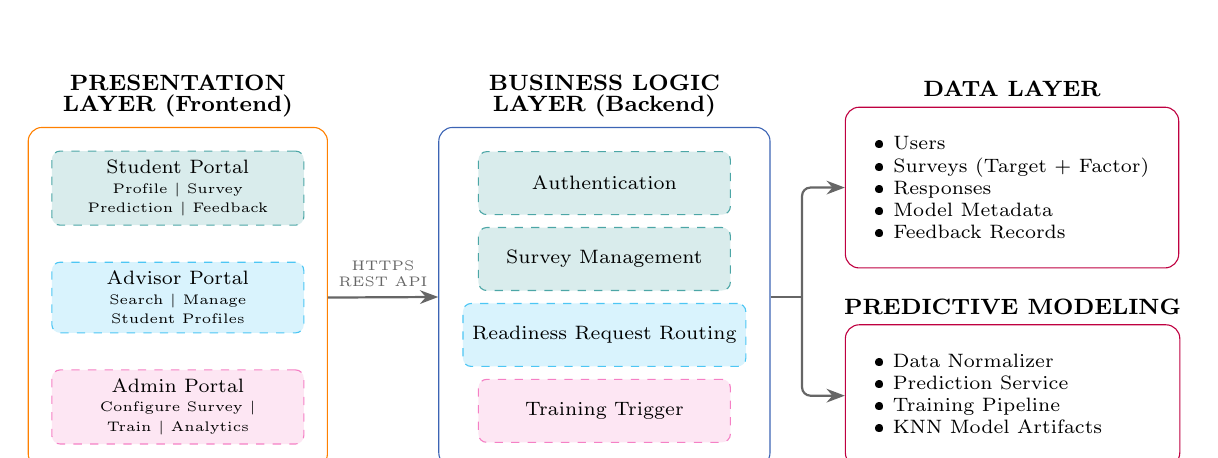
\begin{tikzpicture}[
    node distance=1.5mm,
    box/.style={draw, dashed, rounded corners=3pt, minimum width=32mm, minimum height=8mm, align=center, font=\scriptsize},
    layer/.style={draw, rounded corners=5pt, inner sep=3mm},
    student/.style={box, draw=teal!70, fill=teal!15},
    advisor/.style={box, draw=cyan!70, fill=cyan!15},
    admin/.style={box, draw=magenta!50, fill=magenta!10},
    lbl/.style={font=\footnotesize\bfseries, align=center},
    >=Stealth
]

% Column 2: Business Logic Layer (reference)
\node[student] (auth) {Authentication};
\node[student, below=of auth] (surv) {Survey Management};
\node[advisor, below=of surv] (stage) {Readiness Request Routing};
\node[admin, below=of stage] (train) {Training Trigger};

\begin{scope}[on background layer]
\node[layer, draw=dblue, fit=(auth)(surv)(stage)(train), label={[lbl]above:BUSINESS LOGIC\\[-2pt]LAYER (Backend)}] (biz) {};
\end{scope}

% Column 1: Presentation Layer - create outer box first, then place inner boxes
\path let \p1=(biz.north), \p2=(biz.south), \p3=(biz.west) in
    node[layer, draw=orange,
         minimum height={\y1-\y2},
         minimum width=38mm,
         anchor=north east,
         label={[lbl]above:PRESENTATION\\[-2pt]LAYER (Frontend)}] (pres) at ($(\x3,\y1)+(-14mm,0)$) {};

% Place boxes centered inside pres
\node[student, anchor=north] at ($(pres.north)+(0,-3mm)$) (sp) {Student Portal\\[-1pt]\tiny Profile \textbar{} Survey\\[-1pt]\tiny Prediction \textbar{} Feedback};
\node[advisor] at (pres.center) (ap) {Advisor Portal\\[-1pt]\tiny Search \textbar{} Manage\\[-1pt]\tiny Student Profiles};
\node[admin, anchor=south] at ($(pres.south)+(0,3mm)$) (adm) {Admin Portal\\[-1pt]\tiny Configure Survey \textbar{} \\[-1pt]\tiny Train \textbar{} Analytics};

% Column 3: Data Layer (top) + ML Layer (bottom)
% Position Data Layer at top, aligned with Business Logic Layer outer box
\path let \p1=(biz.north east) in
    node[font=\scriptsize, align=left, anchor=north west] (dlist) at ($(\x1,\y1)+(12mm,0)$) {
        \textbullet\ Users\\
        \textbullet\ Surveys (Target + Factor)\\
        \textbullet\ Responses\\
        \textbullet\ Model Metadata\\
        \textbullet\ Feedback Records
    };

\begin{scope}[on background layer]
\node[layer, draw=purple, fit=(dlist), inner sep=2.5mm, label={[lbl]above:DATA LAYER}] (data) {};
\end{scope}

% Predictive Modeling Layer - align bottom with Business Logic Layer
\path let \p1=(data.west), \p2=(data.east), \p3=(biz.south) in
    node[layer, draw=purple, minimum width={\x2-\x1}, minimum height=18mm, anchor=south west, label={[lbl]above:PREDICTIVE MODELING}] (ml) at (\x1,\y3) {};

\node[font=\scriptsize, align=left, anchor=north west] at ($(ml.north west)+(2.5mm,-2.5mm)$) {
    \textbullet\ Data Normalizer\\
    \textbullet\ Prediction Service\\
    \textbullet\ Training Pipeline\\
    \textbullet\ KNN Model Artifacts
};

% Arrows
\draw[->, thick, black!60] (pres.east) -- (biz.west) node[midway, above, font=\tiny, align=center] {HTTPS\\REST API};
\coordinate (split) at ($(biz.east)+(4mm,0)$);
\draw[thick, black!60] (biz.east) -- (split);
\draw[->, thick, black!60, rounded corners=3pt] (split) |- (data.west);
\draw[->, thick, black!60, rounded corners=3pt] (split) |- (ml.west);

\end{tikzpicture}
}%
\end{figure}

\subsection{Dual-survey architecture}\label{subsec:dualsurvey}

% REV-SUCCESS-001 BEGIN: distinguish longitudinal success from readiness labels.
In this paper, distal \textbf{student success} means persistence after transfer, satisfactory academic progress and credit accumulation, and eventual bachelor's degree completion. These outcomes require longitudinal institutional records and were not observed in the pilot. The current Target Survey score is instead a proximal, self-reported \textbf{readiness composite}. It summarizes students' reported confidence, commitment, time management, and related constructs at one point in time. It is neither an observed success outcome nor evidence that a student will persist or graduate.

Because ACOSUS separates the current readiness label from the information used to estimate it, three terms are central to the design:

\begin{itemize}
    \item \textbf{Target Survey / Readiness Label ($Y$)}: The survey instrument that produces the proximal self-reported readiness composite used as the current model label.
    \item \textbf{Factor Survey / Predictors ($X$)}: The survey instruments that collect information used to make predictions, including academic background, financial circumstances, and logistical constraints. In machine learning terminology, these are \emph{features} or \emph{independent variables}.
    \item \textbf{Constructs}: Psychological or educational concepts (e.g., self-efficacy, institutional commitment) that we operationalize through survey questions. A single Factor Survey may measure multiple constructs.
\end{itemize}

These definitions matter because many of the factors that shape transfer success do not map cleanly onto the information universities already store. Variables such as credit articulation outcomes, transfer shock, belonging, and financial precarity are rarely captured in standard institutional systems \parencite{nguyen2025school}. Advisors also often lack one place to access the information they need; prior work shows that they spend substantial time gathering student data from multiple sources before they can offer useful guidance \parencite{preposttransfer2014}. ACOSUS addresses both issues through a dual-survey architecture that consolidates advisor-facing information and supports later modeling research.

Prior research identifies constructs associated with transfer outcomes, including academic self-efficacy, institutional commitment, social integration, and career clarity \parencite{factoranalysis2023}. Our earlier factor-analysis work grouped related variables into clusters such as academic confidence, time management, financial stability, and support systems \parencite{factoranalysis2023}. ACOSUS uses these constructs to operationalize readiness. The present study does not equate that readiness measure with longitudinal student success.

ACOSUS implements this framework through a Dual-Survey Architecture that separates readiness-label collection from factor collection (Figure~\ref{fig:dualsurvey}). \textbf{Target Surveys} (measuring $Y$) support either a direct 0--100 self-rating or a multi-question instrument whose items are aggregated into a readiness composite. \textbf{Factor Surveys} (measuring $X$) collect academic background, financial circumstances, logistical constraints, and prior interests or experiences.
% REV-SUCCESS-001 END

Factor Surveys standardize transfer-specific information that might otherwise be gathered through inconsistent interviews. Every participating student answers the same question set, supporting cohort-level description and reducing the chance that relevant context is omitted. In the pushed implementation, responses are available in the advisor dashboard, although the efficiency and usability of that workflow have not been formally evaluated.

The architecture also supports flexible study designs through \textbf{survey linkage}, meaning explicit associations between Target and Factor Surveys. Linkage allows future studies to compare predictor sets, add factors, and customize instruments for different cohorts without changing the core infrastructure. The next step transforms raw responses into consistent numeric inputs. We return to linkage when discussing configuration flexibility.

% Figure 2 - Dual-Survey Architecture diagram
\begin{figure}[htbp]
\caption{Dual-Survey Architecture. Target Surveys produce a proximal readiness label ($Y$), and Factor Surveys collect candidate predictors ($X$). The readiness label is not an observed longitudinal student-success outcome.}
\label{fig:dualsurvey}
\centering
\resizebox{0.72\textwidth}{!}{%
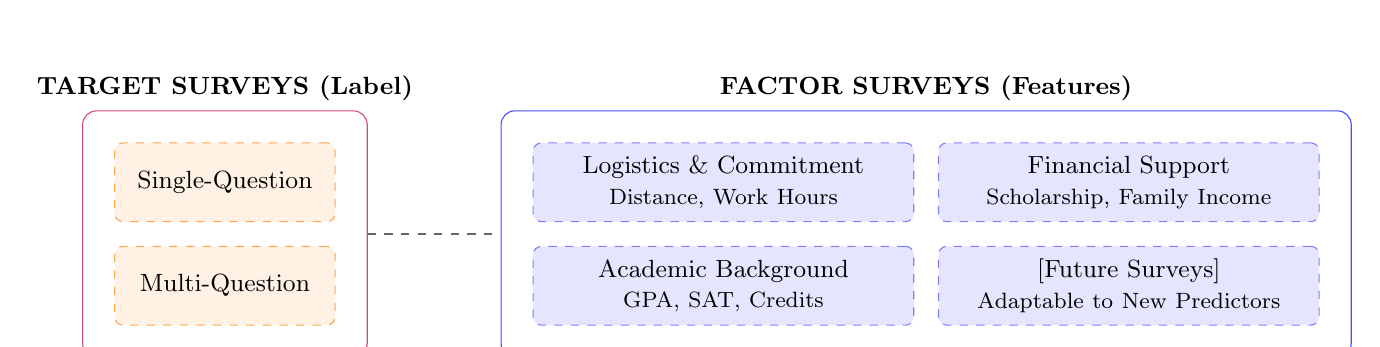
\begin{tikzpicture}[
  box/.style={draw,dashed,rounded corners=3pt,align=center,font=\small},
  target/.style={box,draw=orange!70,fill=orange!10,minimum width=28mm,minimum height=10mm},
  factor/.style={box,draw=blue!50,fill=blue!10,minimum width=48mm,minimum height=10mm,text width=46mm},
  container/.style={draw,rounded corners=5pt,inner sep=4mm}
]
% Target surveys
\node[target] (sq) {Single-Question};
\node[target,below=3mm of sq] (mq) {Multi-Question};
\node[container,draw=purple!70,fit=(sq)(mq),label={[font=\small\bfseries]above:TARGET SURVEYS (Label)}] (tbox) {};

% Factor surveys
\node[factor,right=25mm of sq] (lc) {Logistics \& Commitment\\\footnotesize Distance, Work Hours};
\node[factor,right=3mm of lc] (fs) {Financial Support\\\footnotesize Scholarship, Family Income};
\node[factor,below=3mm of lc] (ab) {Academic Background\\\footnotesize GPA, SAT, Credits};
\node[factor,right=3mm of ab] (fu) {[Future Surveys]\\\footnotesize Adaptable to New Predictors};
\node[container,draw=blue!70,fit=(lc)(fs)(ab)(fu),label={[font=\small\bfseries]above:FACTOR SURVEYS (Features)}] (fbox) {};

% Connection
\draw[black!60,dashed,thick] (tbox.east) -- (fbox.west);
\end{tikzpicture}
}%
\end{figure}

\subsection{Survey data processing}\label{subsec:dataprocessing}

The Target and Factor Survey instruments convert student responses into feature vectors for predictive modeling, following the pipeline shown in Figure~\ref{fig:processing}. Each question corresponds to a success-related factor identified in prior research. Our earlier factor-analysis work linked observable indicators such as scholarship status and commute distance to broader constructs such as financial stability and institutional commitment \parencite{factoranalysis2023}. The purpose of this stage is to move from survey design to a consistent numerical representation that later modeling stages can use.

\subsubsection{Priority weighting}

The deterministic readiness calculation uses question-level \textbf{priority scores} to make the contribution of each response explicit. The current priorities are literature-informed design choices, not coefficients estimated from longitudinal outcomes. They should therefore be interpreted as transparent heuristics whose consequences can be inspected and revised, rather than as empirically validated effects (Table~\ref{tab:priority}).

The priority-weighted aggregation follows a straightforward formulation. For a survey with $n$ questions, where question $i$ has priority score $p_i$, the student selects an option with weightage $w_i^{\text{selected}}$ from a maximum possible $w_i^{\text{max}}$:

\begin{equation}
S = \frac{\sum_{i=1}^{n} \left(\frac{w_i^{\text{selected}}}{w_i^{\text{max}}} \times p_i\right)}{\sum_{i=1}^{n} p_i}
\label{eq:priority}
\end{equation}

This yields a normalized score in $[0, 1]$ that reflects both the selected response and the importance of the corresponding question. We then apply a logistic calibration curve to reduce overconfident predictions at the extremes.

\begin{table}[htbp]
\caption{Example priority score assignments based on literature-informed importance.}
\label{tab:priority}
\centering
\begin{tabular}{@{}p{3.1cm}p{4.5cm}cp{3.5cm}@{}}
\toprule
\textbf{Factor Category} & \textbf{Example Question} & \textbf{Priority} & \textbf{Rationale} \\
\midrule
Academic ~ ~ ~ ~ ~ ~ ~ ~ ~ Self-Efficacy & How confident in your ability to succeed? & 9 & Strong predictor (\parencite{bandura1997}) \\
\midrule
Financial Stability & Expected financial stress impact? & 8 & Affects retention (\parencite{socialcognitive2022}) \\
\midrule
Institutional Commitment & How committed to completing this program? & 9 & Persistence indicator (\parencite{tinto1993}) \\
\midrule
Logistics & Commute distance to university? & 6 & Practical barrier \\
\bottomrule
\end{tabular}
\end{table}

% REV-WEIGHT-001 BEGIN: aggregate sensitivity analysis, not weight validation.
We examined how alternative priority assignments changed the ten available deidentified profiles. Table~\ref{tab:sensitivity} reports equal weights, doubled academic priorities, doubled support and logistics priorities, and one-at-a-time changes of plus or minus 20 percent. Scores use the same weighted aggregation and logistic calibration as the pushed implementation.

\begin{table}[htbp]
\caption{Priority-weight sensitivity across the ten available profiles.}
\label{tab:sensitivity}
\centering
\begin{tabular}{@{}p{3.9cm}rrrr@{}}
\toprule
\textbf{Scenario} & \textbf{Mean} & \textbf{Mean $|\Delta|$} & \textbf{Max $|\Delta|$} & \textbf{$\rho$} \\
\midrule
Baseline priorities & 82.27 & 0.00 & 0.00 & 1.000 \\
Equal weights & 81.10 & 1.77 & 5.24 & 0.988 \\
Double academic priorities & 81.35 & 1.22 & 2.63 & 0.964 \\
Double support/logistics priorities & 81.76 & 1.23 & 3.21 & 0.976 \\
One-at-a-time $\pm20\%$ & -- & 0.34 & 1.23 & $\geq0.988$ \\
\bottomrule
\end{tabular}
\end{table}

The rankings were locally stable for these profiles, although equal weighting changed one score by 5.24 points. This is a sensitivity result, not empirical validation of the baseline priorities or of readiness as a predictor of persistence or completion. Longitudinal outcomes are required to estimate or validate weights.
% REV-WEIGHT-001 END

The next step in processing is to normalize different response types appropriately.

\subsubsection{Data type handling}

Survey responses include different data types, and each type requires an appropriate normalization step before modeling, as summarized in Table~\ref{tab:normalization}. The distinction between \textbf{ordinal} and \textbf{cardinal} data is especially important: ordinal responses (e.g., ``Not confident'' $<$ ``Somewhat confident'' $<$ ``Very confident'') have a meaningful order, whereas cardinal responses (e.g., career aspiration categories) do not imply ranking.

\begin{table}[htbp]
\caption{Normalization strategies for different data types.}
\label{tab:normalization}
\centering
\begin{tabular}{@{}lll@{}}
\toprule
\textbf{Data Type} & \textbf{Example} & \textbf{Normalization Method} \\
\midrule
Ordinal & GPA range: ``3.0--3.5'' & Direct option weightage (e.g., 8/10) \\
Cardinal & Career: ``Industry/Corporate'' & Equal weightage or domain-specific mapping \\
Continuous & SAT score: 1250 & Min-max scaling: $(x - \min)/(\max - \min)$ \\
\bottomrule
\end{tabular}
\end{table}

This type-aware processing preserves the meaning of the responses during feature engineering: ordinal relationships remain ordered, nominal categories are not treated as ranked, and continuous values are scaled appropriately. With this processing in place, ACOSUS can pass standardized inputs to the prediction pipeline. The next subsection explains how that pipeline is designed for settings where only a small amount of institutional data is available at first.

% Figure 3 - Survey Data Processing Pipeline diagram
\begin{figure}[htbp]
\caption{Survey data processing pipeline. Raw responses undergo priority weighting and type-aware normalization to produce standardized feature vectors for readiness scoring and post-pilot model experiments.}
\label{fig:processing}
\centering
\resizebox{0.80\textwidth}{!}{%
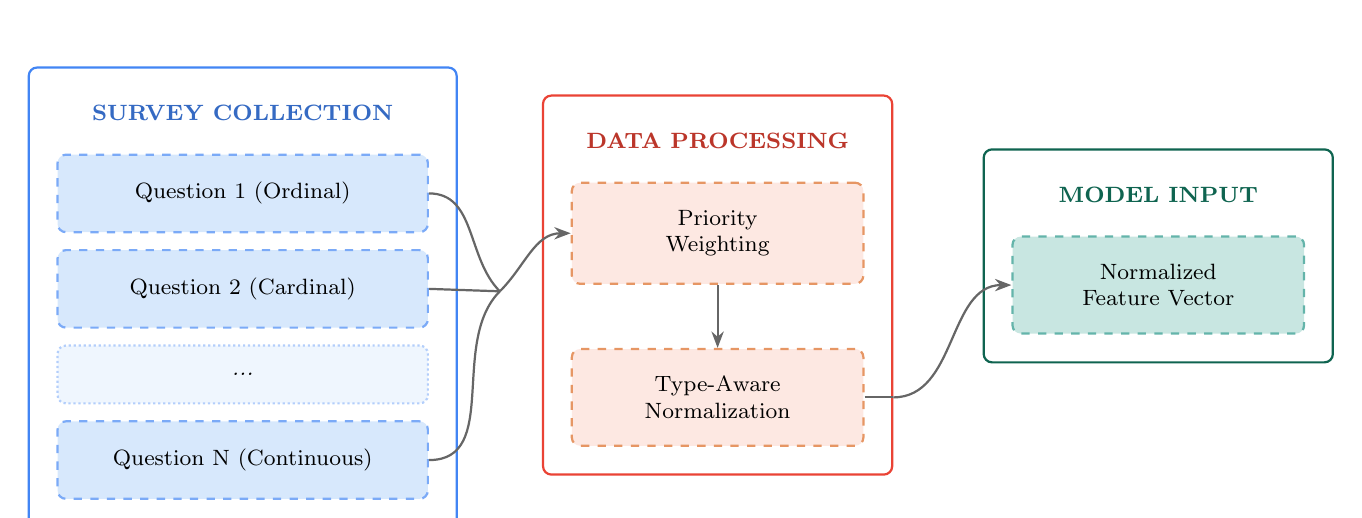
\begin{tikzpicture}[
    node distance=0.35cm,
    inner/.style={rectangle, dashed, thick, rounded corners=3pt, align=center, inner sep=10pt, font=\footnotesize},
    outer/.style={rectangle, thick, rounded corners=3pt, inner sep=6pt},
    arrow/.style={-{Stealth[scale=0.9]}, black!60, thick, rounded corners=6pt},
    arrowline/.style={black!60, thick, rounded corners=6pt}
]

% Survey Collection inner boxes
\node[inner, fill=surveyboxfill, draw=surveyblue!70, text width=4cm, minimum height=0.5cm] (q1) {Question 1 (Ordinal)};
\node[inner, fill=surveyboxfill, draw=surveyblue!70, text width=4cm, minimum height=.5cm, below=0.2cm of q1] (q2) {Question 2 (Cardinal)};
\node[inner, fill=surveyboxfill!40, draw=surveyblue!40, densely dotted, text width=4cm, minimum height=.5cm, below=0.2cm of q2] (qdots) {\textit{...}};
\node[inner, fill=surveyboxfill, draw=surveyblue!70, text width=4cm, minimum height=0.5cm, below=0.2cm of qdots] (qn) {Question N (Continuous)};

% Survey Collection title and outer box
\node[above=0.3cm of q1, font=\footnotesize\bfseries, text=surveyblue!80!black] (survey-title) {SURVEY COLLECTION};
\node[outer, draw=surveyblue, fit=(survey-title)(q1)(q2)(qdots)(qn), inner sep=10pt] (survey-box) {};

% Data Processing inner boxes
\node[inner, fill=processboxfill, draw=processboxborder, text width=3cm, minimum height=1cm, right=1.8cm of q1.east |- q1.south east] (priority) {Priority\\Weighting};
\node[inner, fill=processboxfill, draw=processboxborder, text width=3cm, minimum height=1cm, below=0.8cm of priority] (normalize) {Type-Aware\\Normalization};

% Data Processing title and outer box
\node[above=0.3cm of priority, font=\footnotesize\bfseries, text=processorange!80!black] (process-title) {DATA PROCESSING};
\node[outer, draw=processorange, fit=(process-title)(priority)(normalize), inner sep=10pt] (process-box) {};

% Model Input inner box (centered with process box)
\path (priority.center) -- (normalize.center) coordinate[midway] (process-center);
\node[inner, fill=modelboxfill, draw=modelboxborder, text width=3cm, minimum height=1cm, right=1.5cm of process-box.east, anchor=west] (feature) {Normalized\\Feature Vector};

% Model Input title and outer box
\node[above=0.3cm of feature, font=\footnotesize\bfseries, text=modelgreen] (model-title) {MODEL INPUT};
\node[outer, draw=modelgreen, fit=(model-title)(feature), inner sep=10pt] (model-box) {};

% Arrows from Survey to Priority Weighting (converging)
% Merge point at Q2 level so Q2 has straight horizontal line
\coordinate (merge-point) at ($(survey-box.east)!0.5!(process-box.west)$ |- q2);

% Curved lines from questions converging to merge point, then to priority
\draw[arrowline] (q1.east) to[out=0, in=135] (merge-point);
\draw[arrowline] (q2.east) -- (merge-point);
\draw[arrowline] (qn.east) to[out=0, in=-135] (merge-point);
\draw[arrow] (merge-point) to[out=45, in=180] (priority.west);

% Arrow between Priority and Normalization
\draw[arrow] (priority.south) -- (normalize.north);

% Arrow from Normalization to Feature Vector
\draw[arrowline] (normalize.east) -- (process-box.east |- normalize.east);
\draw[arrow] (process-box.east |- normalize.east) to[out=0, in=180] (feature.west);

\end{tikzpicture}
}%
\end{figure}

\subsection{Implemented foundation components and proposed learning roadmap}\label{subsec:progressive}

After survey responses have been standardized, the immediate implemented value is structured collection and advisor-visible organization. The pushed post-pilot implementation also contains deterministic readiness scoring and a KNN path. The broader progression from limited-data collection to synthetic augmentation and advanced models is a research roadmap, not an evaluated pipeline.

\subsubsection{Three-stage pipeline}

Figure~\ref{fig:pipeline} presents the proposed three-stage roadmap:

\textbf{Foundation Stage.} The implemented survey workflow collects readiness labels and factor responses, and the advisor dashboard organizes them. A KNN component was added after the pilot, but its readiness predictions have not been validated against longitudinal student outcomes.

\textbf{Augmentation Stage.} Future research may test synthetic-data methods only after sufficient real observations exist to evaluate fidelity, privacy, bias, and utility. No synthetic augmentation is active in the pushed implementation.

\textbf{Refinement Stage.} Advanced nonlinear or ensemble models remain future work. Their adoption would require out-of-sample performance, calibration, fairness, and institutional generalizability evidence.

% REV-MODEL-001 BEGIN: active cautious numeric treatment.
We reproduced a leakage-safe leave-one-out diagnostic for the post-pilot KNN using the ten committed deidentified profiles, 17 encoded features, three distance-weighted neighbors, Euclidean distance, and fold-specific standardization. The KNN produced MAE 4.63, RMSE 5.91, and $R^2=-0.26$. A leave-one-out mean baseline produced MAE 4.38, RMSE 5.85, and $R^2=-0.24$. The KNN therefore did not outperform the baseline. These labels are self-reported readiness composites, not persistence, credit accumulation, degree completion, or another longitudinal outcome. The diagnostic does not support a predictive-validity claim.
% Alternative A, methods without metrics: The pushed post-pilot implementation contains a distance-weighted KNN path with standardized inputs. Because the available labels are ten self-reported readiness composites rather than longitudinal outcomes, model performance is not treated as evidence of student-success prediction.
% Alternative B, complete deferral: Predictive model evaluation is deferred until longitudinal outcomes and a sufficiently large independent sample are available.
% REV-MODEL-001 END

The stage structure is retained as a roadmap for future experiments. It does not imply automatic transitions, validated synthetic augmentation, or production use of advanced models.

% Figure 4 - Three-Stage Progressive Pipeline diagram
\begin{figure}[htbp]
\caption{Proposed three-stage research roadmap. Only structured data collection, advisor-visible profiles, deterministic readiness scoring, and a post-pilot KNN path are currently implemented. Augmentation, refinement, automatic transitions, and continuous improvement remain future work.}
\label{fig:pipeline}
\centering
\resizebox{\textwidth}{!}{%
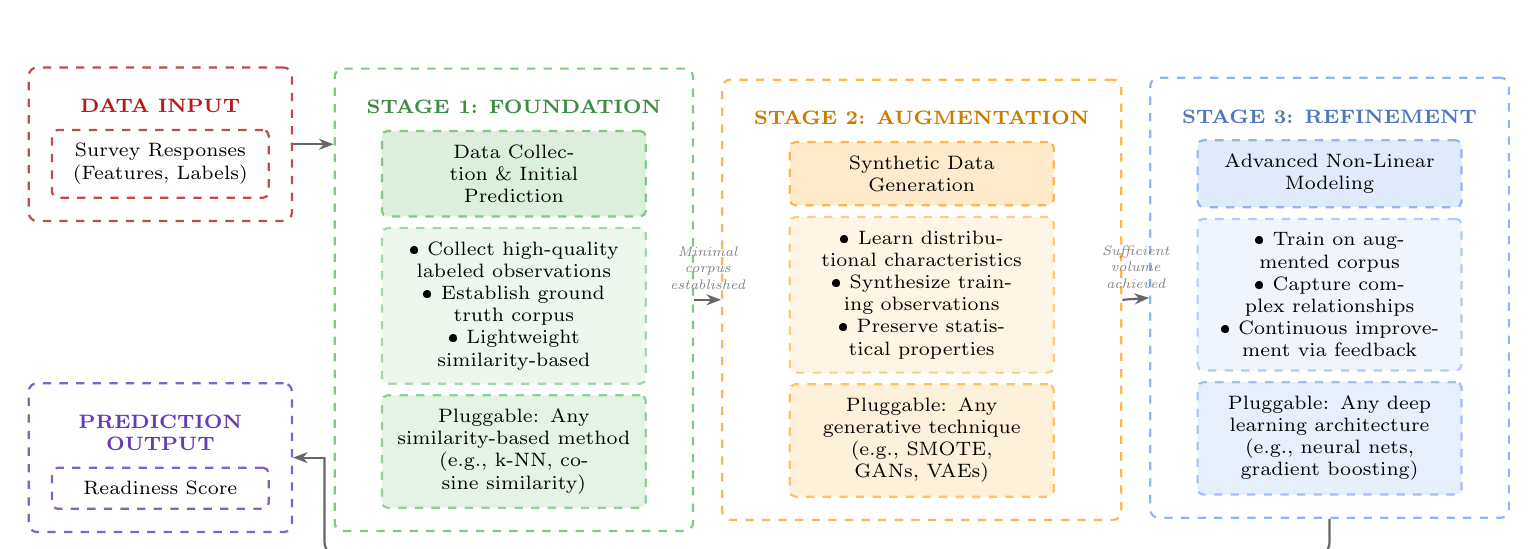
\begin{tikzpicture}[
    node distance=0.3cm,
    inner/.style={rectangle, dashed, thick, rounded corners=2pt, align=center, inner sep=5pt, font=\scriptsize},
    outer/.style={rectangle, dashed, thick, rounded corners=3pt, inner sep=8pt},
    header/.style={inner, fill=#1!20, draw=#1!70},
    content/.style={inner, fill=#1!10, draw=#1!50},
    plug/.style={inner, fill=#1!15, draw=#1!60},
    arrow/.style={-{Stealth[scale=0.8]}, black!60, thick},
    lbl/.style={font=\tiny\itshape, text=black!50, align=center}
]

% Stage 1 inner boxes
\node[header=stage1, text width=3cm, minimum height=0.8cm] (s1-head) {Data Collection \& Initial\\Prediction};
\node[content=stage1, below=0.12cm of s1-head, text width=3cm, minimum height=1.4cm] (s1-content) {
    \textbullet\ Collect high-quality labeled observations\\
    \textbullet\ Establish ground truth corpus\\
    \textbullet\ Lightweight similarity-based
};
\node[plug=stage1, below=0.12cm of s1-content, text width=3cm, minimum height=0.9cm] (s1-plug) {Pluggable: Any\\similarity-based method\\(e.g., k-NN, cosine similarity)};
\node[above=0.08cm of s1-head, font=\scriptsize\bfseries, text=stage1!80!black] (s1-title) {STAGE 1: FOUNDATION};
\node[outer, draw=stage1!70, fit=(s1-title)(s1-head)(s1-content)(s1-plug)] (stage1-box) {};

% Stage 2 inner boxes
\node[header=stage2, right=1.8cm of s1-head, text width=3cm, minimum height=0.8cm] (s2-head) {Synthetic Data\\Generation};
\node[content=stage2, below=0.12cm of s2-head, text width=3cm, minimum height=1.4cm] (s2-content) {
    \textbullet\ Learn distributional characteristics\\
    \textbullet\ Synthesize training observations\\
    \textbullet\ Preserve statistical properties
};
\node[plug=stage2, below=0.12cm of s2-content, text width=3cm, minimum height=0.9cm] (s2-plug) {Pluggable: Any\\generative technique\\(e.g., SMOTE, GANs, VAEs)};
\node[above=0.08cm of s2-head, font=\scriptsize\bfseries, text=stage2!80!black] (s2-title) {STAGE 2: AUGMENTATION};
\node[outer, draw=stage2!70, fit=(s2-title)(s2-head)(s2-content)(s2-plug)] (stage2-box) {};

% Stage 3 inner boxes
\node[header=stage3, right=1.8cm of s2-head, text width=3cm, minimum height=0.8cm] (s3-head) {Advanced Non-Linear\\Modeling};
\node[content=stage3, below=0.12cm of s3-head, text width=3cm, minimum height=1.4cm] (s3-content) {
    \textbullet\ Train on augmented corpus\\
    \textbullet\ Capture complex relationships\\
    \textbullet\ Continuous improvement via feedback
};
\node[plug=stage3, below=0.12cm of s3-content, text width=3cm, minimum height=0.9cm] (s3-plug) {Pluggable: Any deep\\learning architecture\\(e.g., neural nets, gradient boosting)};
\node[above=0.08cm of s3-head, font=\scriptsize\bfseries, text=stage3!80!black] (s3-title) {STAGE 3: REFINEMENT};
\node[outer, draw=stage3!70, fit=(s3-title)(s3-head)(s3-content)(s3-plug)] (stage3-box) {};

% Pipeline title (centered above stages)
% \path (stage1-box.north west) -- (stage3-box.north east) coordinate[midway] (pipeline-center);
% \node[above=0.6cm of pipeline-center, font=\small\bfseries, text=pipelineborder] (pipeline-title) {ACOSUS THREE-STAGE PROGRESSIVE PIPELINE};

% Pipeline outer box
% \begin{scope}[on background layer]
% \node[outer, draw=pipelineborder, fit=(pipeline-title)(stage1-box)(stage2-box)(stage3-box), inner sep=12pt] (pipeline) {};
% \end{scope}

% Input box (outer box top aligned with Stage 1 outer box top)
\node[font=\scriptsize\bfseries, text=inputred, anchor=north] (input-title) at ([xshift=-2.2cm, yshift=-8pt]stage1-box.north west) {DATA INPUT};
\node[inner, fill=white, draw=inputred!80, text width=2.4cm, below=0.08cm of input-title] (input-inner) {Survey Responses\\(Features, Labels)};
\node[outer, draw=inputred!80, fit=(input-title)(input-inner)] (input-box) {};

% Output box (outer box bottom aligned with Stage 1 outer box bottom)
\node[inner, fill=white, draw=outputviolet!80, text width=2.4cm, anchor=south] (output-inner) at ([xshift=-2.2cm, yshift=8pt]stage1-box.south west) {Readiness Score};
\node[above=0.08cm of output-inner, font=\scriptsize\bfseries, text=outputviolet, align=center] (output-title) {PREDICTION\\ OUTPUT};
\node[outer, draw=outputviolet!80, fit=(output-title)(output-inner)] (output-box) {};

% Arrows
\draw[arrow] (input-box.east) -- (stage1-box.west |- input-box.east);
\draw[arrow] (stage1-box.east) -- node[lbl, above] {Minimal\\corpus\\established} (stage2-box.west);
\draw[arrow] (stage2-box.east) -- node[lbl, above] {Sufficient\\volume\\achieved} (stage3-box.west);

% Feedback arrow
\coordinate (turn1) at ([yshift=-0.5cm]stage3-box.south);
\coordinate (turn2) at (turn1 -| output-box.east);
\coordinate (turn3) at ([xshift=0.4cm]output-box.east);
\draw[black!60, thick, rounded corners=6pt] (stage3-box.south) -- (turn1) -- (turn1 -| turn3) -- (turn3);
\draw[arrow] (turn3) -- (output-box.east);

\end{tikzpicture}
}%
\end{figure}

\subsection{Configuration flexibility}\label{subsec:config}

The current configuration system supports survey definitions and explicit linkage between Target and Factor Surveys. The later-stage configuration categories described below are design requirements for the research roadmap, not evidence of completed automated orchestration.

\textbf{Survey Linkage:} The implemented dual-survey architecture uses explicit linkage settings. A single Target Survey readiness label ($Y$) may be linked to multiple Factor Surveys (candidate predictor sets $X_1, X_2, X_3$). Figure~\ref{fig:linkage} shows the implemented linkage and the post-pilot KNN path. This arrangement supports several future study designs:

\begin{enumerate}
    \item \textbf{Comparative predictor analysis:} researchers could deploy alternative Factor Surveys to the same cohort and compare their validity once suitable outcomes exist;
    \item \textbf{Longitudinal adaptability:} as research identifies new predictors of transfer success, new Factor Surveys can be added without disrupting existing data collection or invalidating earlier comparisons;
    \item \textbf{Cohort customization:} different academic programs can deploy program-specific Factor Surveys while maintaining a common outcome measure through shared Target Surveys.
\end{enumerate}

% Figure 5 - Dual-Survey Architecture with Linkage
\begin{figure}[htbp]
\caption{Implemented survey linkage and post-pilot KNN path. Target Surveys provide readiness labels and Factor Surveys provide candidate features. The diagram does not imply validated prediction of longitudinal outcomes.}
\label{fig:linkage}
\centering
\resizebox{0.67\textwidth}{!}{%
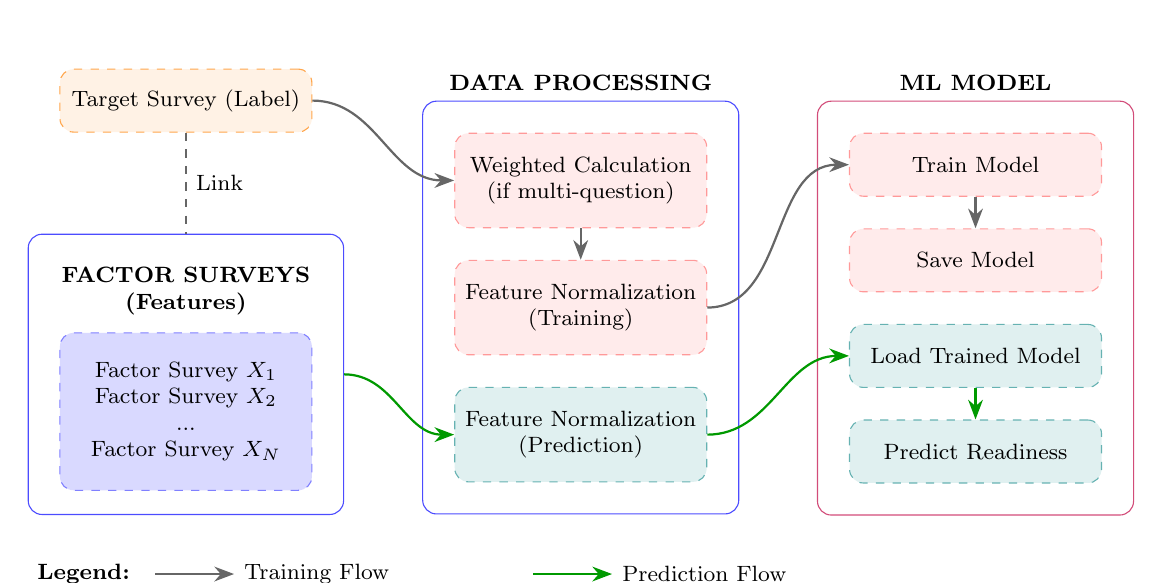
\begin{tikzpicture}[
  box/.style={draw,dashed,rounded corners=5pt,align=center,font=\footnotesize},
  container/.style={draw,rounded corners=5pt,inner sep=4mm},
  % Training flow styles (warm/salmon hues)
  trainbox/.style={box,draw=red!40,fill=red!8},
  trainarr/.style={black!60,thick,-{Stealth[length=2.5mm]}},
  % Prediction flow styles (cool/teal hues)
  predbox/.style={box,draw=teal!60,fill=teal!12},
  predarr/.style={green!60!black,thick,-{Stealth[length=2.5mm]}}
]
% Left column - Target Survey
\node[box,draw=orange!70,fill=orange!10,minimum width=32mm,minimum height=8mm] (target) {Target Survey (Label)};

% Middle column - Data Processing
\node[trainbox,minimum width=32mm,minimum height=12mm,right=18mm of target.south east,anchor=north west] (weighted) {Weighted Calculation\\(if multi-question)};
\node[trainbox,minimum width=32mm,minimum height=12mm,below=4mm of weighted] (normtrain) {Feature Normalization\\(Training)};
\node[predbox,minimum width=32mm,minimum height=12mm,below=4mm of normtrain] (normpred) {Feature Normalization\\(Prediction)};
\node[container,draw=blue!70,fit=(weighted)(normtrain)(normpred),label={[font=\footnotesize\bfseries]above:DATA PROCESSING}] (dbox) {};

% Left column - Factor Surveys (aligned to dbox bottom)
\node[box,draw=blue!50,fill=blue!15,minimum width=32mm,minimum height=20mm,anchor=south] at ([yshift=3mm]target.south|-dbox.south) (factors) {Factor Survey $X_1$\\Factor Survey $X_2$\\...\\Factor Survey $X_N$};
\node[font=\footnotesize\bfseries,align=center,above=1mm of factors] (flabel) {FACTOR SURVEYS\\(Features)};
\node[container,draw=blue!70,inner sep=3mm,fit=(factors)(flabel)] (fbox) {};

% Link between target and factor surveys
\draw[black!60,dashed,thick] (target.south) -- node[right,font=\footnotesize,black]{Link} (fbox.north);

% Right column - ML Model (Training flow on top, Prediction flow on bottom)
\node[trainbox,minimum width=32mm,minimum height=8mm,right=18mm of weighted.north east,anchor=north west] (train) {Train Model};
\node[trainbox,minimum width=32mm,minimum height=8mm,below=4mm of train] (save) {Save Model};
\node[predbox,minimum width=32mm,minimum height=8mm,below=4mm of save] (load) {Load Trained Model};
\node[predbox,minimum width=32mm,minimum height=8mm,below=4mm of load] (predict) {Predict Readiness};
\node[container,draw=purple!70,fit=(train)(save)(load)(predict),label={[font=\footnotesize\bfseries]above:ML MODEL}] (mbox) {};

% Training Flow Arrows (gray)
\draw[trainarr] (target.east) to[out=0,in=180] (weighted.west);
\draw[trainarr] (weighted.south) -- (normtrain.north);
\draw[trainarr] (normtrain.east) to[out=0,in=180] (train.west);
\draw[trainarr] (train.south) -- (save.north);

% Prediction Flow Arrows (green)
\draw[predarr] (fbox.east) to[out=0,in=180] (normpred.west);
\draw[predarr] (normpred.east) to[out=0,in=180] (load.west);
\draw[predarr] (load.south) -- (predict.north);

% Legend (horizontal layout)
\node[below=5mm of fbox.south west,anchor=north west,font=\footnotesize\bfseries] (legendlabel) {Legend:};
\draw[trainarr] ([xshift=2mm]legendlabel.east) -- ++(10mm,0) node[right,font=\footnotesize,black] {Training Flow};
\node[right=50mm of legendlabel.east,anchor=west] (predlegendstart) {};
\draw[predarr] (predlegendstart.west) -- ++(10mm,0) node[right,font=\footnotesize,black] {Prediction Flow};
\end{tikzpicture}
}%
\end{figure}

The remaining three categories describe future work for the proposed roadmap:

\textbf{Phase Transition Thresholds.} Future work must define evidence-based thresholds and transition criteria. Automatic stage transitions are not implemented.

\textbf{Algorithm Selection:} Later experiments may compare compatible algorithms, but synthetic and advanced-model options must not be treated as implemented or beneficial until they are evaluated on appropriate real outcomes.

\textbf{Hyperparameter Tuning:} The KNN implementation exposes core settings such as neighbor count and distance metric. Broader generation, network, and training schedules remain proposed.

These roadmap elements identify a modular direction for later research. They do not establish predictive performance, safe augmentation, or cross-institutional portability.

%%%%%%%%%%%%%%%%%%%%%%%%%%%%%%%%%%%%%%%%%%%%%%%%%
% SECTION 4: EVALUATION
%%%%%%%%%%%%%%%%%%%%%%%%%%%%%%%%%%%%%%%%%%%%%%%%%
\section{Evaluation}\label{sec:evaluation}

To assess the feasibility of the student-facing survey workflow, we conducted a pilot with transfer students recruited from six public U.S. universities. This section reports student perceptions of the workflow. It does not evaluate predictive validity, advisor dashboard usability, longitudinal outcomes, fairness, or institutional deployment.

\subsection{Study design}\label{subsec:studydesign}

% \subsubsection{Participants}

% __ALT_PHRASING__: Study Design participating-institutions sentence (active
% version below is recommended Option A: "from six public universities in the
% United States"). Alternative phrasings retained for reviewer consideration:
%
% Option B (leverages the MSI/HSI alignment with the paper's underrepresented-
% students framing):
%   Ten transfer students ($N=10$) participated, recruited from six public
%   universities in the United States, several of which are designated
%   minority-serving institutions whose student populations align with the
%   underrepresented groups the system is designed to support.
%
% Option C (names institutions explicitly):
%   Ten transfer students ($N=10$) participated, drawn from six public
%   universities in the United States: Northeastern Illinois University,
%   the University of Houston-Downtown, Texas A\&M University-Victoria,
%   SUNY Old Westbury, Cal Poly Humboldt, and the University of Texas at
%   El Paso.
Ten transfer students ($N=10$) from six public universities in the United States participated in the study. Participants were recruited by email and enrolled after providing informed consent. All were active transfer students in computing-related majors. At pilot time, no predictive model had been trained or shown to participants. The evaluated function was structured collection through the Factor and Target Survey instruments. Participants then completed a feedback survey through Qualtrics. The study protocol received Institutional Review Board (IRB) approval before data collection began. Recruitment across six universities describes participant origins only and is not multi-institutional validation of ACOSUS.

\subsection{Evaluation instruments}\label{subsec:instruments}

The feedback survey was based on the Technology Acceptance Model (TAM) framework \parencite{davis1989} and was used to assess participants' perceptions of the data collection experience. It included 5-point Likert-scale items measuring Perceived Usefulness, Perceived Ease of Use, and Behavioral Intention, along with open-ended questions about interface difficulties, helpful features, missing capabilities, and redesign suggestions. Table~\ref{tab:constructs} presents the constructs and example items.

\begin{table}[htbp]
\caption{Feedback survey constructs and items.}
\label{tab:constructs}
\centering
\begin{tabular}{@{}lp{8cm}@{}}
\toprule
\textbf{Construct} & \textbf{Example Item} \\
\midrule
Perceived Usefulness (PU) & ``Using this AI counseling system enables me to accomplish tasks more quickly than other advising methods.'' \\
Perceived Ease of Use (PEOU) & ``Learning to operate this AI counseling system was easy for me.'' \\
Behavioral Intention & ``How likely are you to continue using this system for academic planning?'' \\
\bottomrule
\end{tabular}
\end{table}

Open-ended questions captured qualitative feedback on interface difficulties, helpful features, missing capabilities, and redesign suggestions.

\subsection{Quantitative results}\label{subsec:quantresults}

\subsubsection{TAM construct scores}

% __ALT_PHRASING__: TAM Construct Scores opening paragraph. The active version
% (recommended Option A) is below; alternative phrasings retained for reviewer
% consideration:
%
% Option B (frames the spread as expected rather than as a weakness):
%   The TAM-based measures showed positive endorsement on perceived ease of use
%   and perceived usefulness, with the expected differences across respondents
%   in how strongly each construct was endorsed. Because this evaluation was
%   conducted during the foundation phase, before any predictive output had
%   been generated for participants, the scores reflect participants'
%   experience of the data-collection workflow and interface rather than the
%   system's predictive utility. Lower ratings on usefulness should therefore
%   be read as a reflection of the system's current functionality at the
%   foundation phase rather than as evidence against the underlying design.
%
% Option C (most measured, fewest adjectives):
%   Participants endorsed perceived ease of use and perceived usefulness
%   positively across the TAM dimensions. Because this evaluation was conducted
%   during the foundation phase, before any predictive output had been
%   generated for participants, the scores reflect participants' experience of
%   the data-collection workflow and interface rather than the system's
%   predictive utility. Lower ratings on usefulness should therefore be read
%   as a reflection of the system's current functionality at the foundation
%   phase rather than as evidence against the underlying design.
The TAM-based measures showed high average perceived ease of use and more moderate, dispersed perceived usefulness (Table~\ref{tab:results}). Because no predictive output was shown, these scores concern the data-collection workflow and interface rather than predictive utility.

\begin{table}[htbp]
\caption{Summary statistics for evaluation metrics (5-point Likert scale).}
\label{tab:results}
\centering
\begin{tabular}{@{}lcccc@{}}
\toprule
\textbf{Metric} & \textbf{Mean} & \textbf{SD} & \textbf{Min} & \textbf{Max} \\
\midrule
Perceived Usefulness (PU) & 3.37 & 1.29 & 1 & 5 \\
Perceived Ease of Use (PEOU) & 4.13 & 1.05 & 1 & 5 \\
Likelihood to Continue & 3.12 & 1.89 & 1 & 5 \\
Likelihood to Recommend & 3.00 & 1.77 & 1 & 5 \\
\bottomrule
\multicolumn{5}{@{}p{0.92\columnwidth}@{}}{\textit{Note.} Behavioral-intention items have $N=8$; two participants did not provide a usable rating.} \\
\bottomrule
\end{tabular}
\end{table}

% Figure 6 - TAM construct scores
\begin{figure}[htbp]
\caption{TAM construct scores ($N=10$). Perceived Ease of Use was the highest-rated TAM construct ($M=4.13$), while Perceived Usefulness was lower and more dispersed ($M=3.37$).}
\label{fig:tam}
\centering

\includegraphics[width=0.72\textwidth]{infographics/fig1_tam_metrics.png}
\end{figure}

As Figure~\ref{fig:tam} shows, Perceived Ease of Use received the highest mean among the TAM constructs ($M=4.13$, $SD=1.05$), indicating positive agreement that the system is easy to learn and use, with relatively consistent responses across participants. Perceived Usefulness was lower and more dispersed ($M=3.37$, $SD=1.29$), suggesting that participants saw the system as easy to operate but were less uniformly convinced of its usefulness for their own advising needs.

\subsubsection{Behavioral intention}

% Figure 7 - Behavioral intention metrics
\begin{figure}[htbp]
\caption{Behavioral intention ($N=8$). Likelihood to Continue ($M=3.12$) was slightly higher than Likelihood to Recommend ($M=3.00$); both showed substantial variance across respondents ($SD\approx1.8$).}
\label{fig:behavioral}
\centering

\includegraphics[width=0.78\textwidth]{infographics/fig4_behavioral_intention.png}
\end{figure}

Behavioral intention was the weakest dimension in the evaluation (Figure~\ref{fig:behavioral}). Likelihood to Continue was moderate on average ($M=3.12$, $SD=1.89$), and Likelihood to Recommend was slightly lower and similarly dispersed ($M=3.00$, $SD=1.77$). Values outside the 1-to-5 scale were treated as missing, leaving eight usable ratings for each item. The distributions were bimodal, motivating an exploratory subgroup comparison.

% REV-BIMODAL-001 BEGIN: aggregate exploratory subgroup analysis.
For each respondent, we averaged the available behavioral-intention items. We classified means of 4 or higher as enthusiastic, 2 or lower as skeptical, and values between those thresholds as intermediate. One respondent was missing both items. Table~\ref{tab:subgroups} reports aggregate means only.

\begin{table}[htbp]
\caption{Exploratory behavioral-intention subgroup means.}
\label{tab:subgroups}
\centering
\begin{tabular}{@{}lrrrrrrr@{}}
\toprule
\textbf{Group} & \textbf{$N$} & \textbf{PU} & \textbf{PEOU} & \textbf{Accuracy} & \textbf{Alignment} & \textbf{Relevance} & \textbf{Actionability} \\
\midrule
Enthusiastic & 3 & 4.83 & 5.00 & 4.67 & 4.67 & 4.67 & 5.00 \\
Skeptical & 4 & 2.71 & 3.62 & 2.25 & 2.00 & 2.25 & 2.50 \\
Intermediate & 2 & 2.92 & 3.75 & 4.50 & 3.00 & 2.50 & 3.00 \\
Missing both items & 1 & 2.50 & 4.33 & 4.00 & -- & 3.00 & 2.00 \\
\bottomrule
\end{tabular}
\end{table}

Enthusiastic respondents rated both usability and perceived advising value highly. Skeptical respondents still rated ease of use above the scale midpoint but reported lower usefulness, accuracy, alignment, relevance, and actionability. Their open-ended comments emphasized missing course or prerequisite analysis, deeper career exploration, or a preference for human advising. Given the very small groups, these comparisons are descriptive only. No significance tests were performed, and the pattern cannot support population-level conclusions.
% REV-BIMODAL-001 END

\subsection{Qualitative findings}\label{subsec:qualfindings}

Open-ended responses yielded five main themes, whose frequencies are shown in Figure~\ref{fig:themes} and whose representative quotes appear in Table~\ref{tab:themes}.

% Figure 8 - Qualitative theme distribution
\begin{figure}[htbp]
\caption{Qualitative theme distribution ($N$=10). Feature Requests was the most frequent theme (7 mentions), followed by UI/Navigation Positive (6), No Issues Reported (5), Assessment \& Exploration Value (4), and a single expression of Preference for Human Advising (1).}
\label{fig:themes}
\centering

\includegraphics[width=0.72\textwidth]{infographics/fig6_qualitative_themes.png}
\end{figure}

\begin{table}[htbp]
\caption{Qualitative themes and representative responses ($N=10$).}
\label{tab:themes}
\centering
\begin{tabular}{@{}lcp{7cm}@{}}
\toprule
\textbf{Theme} & \textbf{Count} & \textbf{Representative Quote} \\
\midrule
Feature Requests & 7 & ``Make it tailored more towards individual users and their specific situation''; ``Better analysis of prerequisites to allow for registration'' \\
UI/Navigation Positive & 6 & ``The UI navigation is very user friendly''; ``All the interface of the website was very intuitive to interact with'' \\
No Issues Reported & 5 & ``No feature was missing, my experience was great''; ``None, everything was clear'' \\
Assessment \& Exploration Value & 4 & ``The assessment is fun and helpful to me''; ``Career exploration'' \\
Preference for Human Advising & 1 & ``I have never had a problem with a human advisor. Please don't replace a human being with AI'' \\
\bottomrule
\end{tabular}
\end{table}

\textbf{Feature Requests} was the most frequent theme. Several participants asked for tighter personalization, prerequisite analysis, and more answer options. \textbf{UI/Navigation Positive} was the next most common theme and was consistent with PEOU being the highest-rated TAM construct ($M=4.13$). \textbf{No Issues Reported} captured responses indicating that the workflow was clear. \textbf{Assessment \& Exploration Value} captured perceived value for self-assessment and career exploration even though no predictions were shown. A fifth theme came from one skeptical participant who preferred human advising and asked that AI not replace an advisor. This isolated comment reinforces the intended role of ACOSUS as support for, rather than a substitute for, human advising.

Outside the formal study, the project received informal comments from academic advisors. These comments suggested potential value in student preparation and a consolidated advising hub, but they were not collected through a defined advisor sample or usability protocol. We therefore do not treat them as evaluation evidence. Formal advisor workflow and usability testing remains future work.

% __ALT_PHRASING__: Advisor feedback final sentence (the second sentence of the
% paragraph above is the recommended Option A). Alternative phrasings retained
% for reviewer consideration:
%
% Option B (drops the template idea entirely; keeps preparedness and hub as
% separate observations):
%   They also observed that the system could encourage student preparedness
%   for advising meetings and that consolidating its captured information into
%   a single advising hub would strengthen its fit with existing advising
%   workflows.
%
% Option C (closest to the advisor's own framing, with "for example" softening
% the template):
%   They also suggested that the system could help students prepare for
%   advising meetings, for example through a preparation template, and noted
%   that consolidating its captured information into a single advising hub
%   would strengthen its fit with advising workflows.

%%%%%%%%%%%%%%%%%%%%%%%%%%%%%%%%%%%%%%%%%%%%%%%%%
% SECTION 5: CONCLUSION AND FUTURE WORK
%%%%%%%%%%%%%%%%%%%%%%%%%%%%%%%%%%%%%%%%%%%%%%%%%
\section{Conclusion and Future Work}\label{sec:conclusion}

This paper presented the design and feasibility evaluation of ACOSUS, a structured advising platform for transfer students in computing majors. Its near-term purpose is to reduce fragmented information through consistent transfer-specific data collection and advisor-visible profiles.

%\textbf{Summary of Contributions.} 
Our primary contributions are the implemented dual-survey workflow, structured advisor-facing organization, and a student pilot that documents both ease of use and variation in perceived advising value. The pilot evaluated data collection, not the dashboard or prediction. A deterministic readiness score and KNN path were implemented after the pilot, but the KNN did not outperform a leave-one-out mean baseline on the ten readiness labels.

%\textbf{Limitations and Current Status.} 
% REV-LIMITS-001 BEGIN: explicit evidence limitations.
The pilot's small sample ($N=10$), voluntary enrollment, and cross-sectional design sharply limit generalizability. The study contains no observed persistence, satisfactory-progress, credit-accumulation, or bachelor's-completion outcomes. It provides no fairness analysis, no formal advisor dashboard usability evaluation, and no institutional deployment or multi-institutional validation. Participants came from six universities, but the platform was not deployed and independently evaluated at those six institutions. The current readiness composite is self-reported and must not be interpreted as observed student success.
% REV-LIMITS-001 END

%\textbf{Future Work.} 
Future work should first evaluate the advisor dashboard in real advising workflows and connect readiness measures to longitudinal institutional outcomes. Only then should larger studies assess out-of-sample performance, calibration, subgroup fairness, and generalizability across independently deployed institutions. Synthetic augmentation, advanced models, automatic stage transitions, and narrative explanations remain research possibilities rather than current capabilities.

The present evidence supports ACOSUS as a feasible structured data-collection design. It does not yet establish that ACOSUS predicts or improves longitudinal student success.

%%%%%%%%%%%%%%%%%%%%%%%%%%%%%%%%%%%%%%%%%%%%%%%%%
% ACKNOWLEDGMENT
%%%%%%%%%%%%%%%%%%%%%%%%%%%%%%%%%%%%%%%%%%%%%%%%%

\section{Acknowledgments}
% This research was supported by the National Science Foundation (NSF) CISE-MSI award CNS-2219623 and an ASEE CyBR-MSI mini-grant under NSF award CNS-2139136. 

This material is based upon work supported by the National Science Foundation under Grant No. CNS-2219623.

%%%%%%%%%%%%%%%%%%%%%%%%%%%%%%%%%%%%%%%%%%%%%%%%%
% BIBLIOGRAPHY
%%%%%%%%%%%%%%%%%%%%%%%%%%%%%%%%%%%%%%%%%%%%%%%%%
\begin{sloppypar}
\printbibliography[title={REFERENCES}]
\end{sloppypar}

\end{document}
